\documentclass[a4paper,12pt]{article}
\usepackage[utf8]{inputenc}
\usepackage{longtable}
\usepackage{geometry}
\usepackage{hyperref}
\usepackage{array}
\usepackage{caption}
\usepackage{booktabs}
\geometry{margin=1in}
\usepackage{graphicx}
\usepackage{float}
\usepackage{hyperref}

\title{Software Requirements Specification\\Taxi Tap by Git It Done}
\date{}

\begin{document}

\maketitle

\begin{figure}[H]
  \centering
  
\includegraphics[width=0.5\textwidth]{LogoGroup.png} 
\end{figure}

\begin{figure}[H]
  \centering
  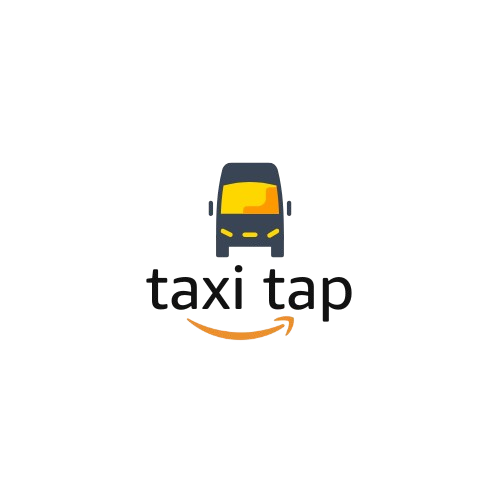
\includegraphics[width=0.5\textwidth]{LogoTaxiTap.png} 
\end{figure}

\newpage

\tableofcontents
\newpage

\section{Introduction}
Taxi Tap is a mobile platform designed to revolutionize South Africa’s minibus taxi industry by digitizing route information, eliminating the need for constant hooting, and creating a semi-structured booking system while preserving the flexibility that makes taxis an essential mode of transport. The system connects passengers and taxi operators through a location-aware mobile application that facilitates taxi requests, communicates passenger locations, and provides real-time vehicle tracking – all without fundamentally changing the existing system's multi-passenger, flexible route nature.

\section{User Characteristics}

The users of the Taxi Tap system are expected to fit into the following groups:

\subsection{Driver User Characteristics}

\begin{table}[H]
\centering
\begin{tabular}{|p{5cm}|p{10cm}|}
\hline
\textbf{Attribute} & \textbf{Description} \\
\hline
Familiarity with Mobile Technology & Varies widely; some drivers may be tech-comfortable, while others may struggle with apps. \\
\hline
Access to Reliable Internet and Data & Often limited or inconsistent; drivers operate in areas with poor signal or expensive data costs. \\
\hline
Preferred Language and Communication Style & Preference for local languages (e.g. Zulu, Xhosa, Sesotho). \\
\hline
Attention Capacity While Driving & App must require minimal taps and distractions to ensure safe usage while driving. \\
\hline
Trust and Skepticism Toward New Technology & Some skepticism exists due to concerns about surveillance, manipulation, or job security. \\
\hline
Goals and Incentives for Using the App & Seeking more passengers, quicker pickups, and less idle time, while maintaining their routine. \\
\hline
\end{tabular}
\caption{Driver User Characteristics and Considerations}
\label{tab:driver-characteristics}
\end{table}

\subsection{Passenger User Characteristics}

\begin{table}[H]
\centering
\begin{tabular}{|p{5cm}|p{10cm}|}
\hline
\textbf{Attribute} & \textbf{Description} \\
\hline
Digital Literacy & Ranges from students and workers (tech-savvy) to commuters with limited app experience. \\
\hline
Access to Reliable Internet and Data & Frequently encounters low or no connectivity, especially in transit. \\
\hline
Reasons for Using the Platform & Seeks reliable transport, less waiting, and a safer way to locate and use taxis. \\
\hline
Preferred Language and Communication Style & May prefer local languages (e.g. Zulu, Xhosa, Sesotho). \\
\hline
App Usage Context (Where \& When) & Often uses the app in crowded, noisy, or busy settings like taxi ranks. \\
\hline
Concerns Around Trust and Safety & Wants to be sure drivers are legitimate and that their location and personal data are protected. \\
\hline
Platform Interaction Needs & Needs to discover taxis, request rides, track driver arrival, and receive ride notifications. \\
\hline
\end{tabular}
\caption{Commuter User Characteristics and Considerations}
\label{tab:commuter-characteristics}
\end{table}

\section{User Stories}

\subsection{Passenger User Stories}

\begin{longtable}{|p{4cm}|p{6cm}|p{5cm}|}
\hline
\textbf{User Story} & \textbf{Acceptance Criteria} & \textbf{Definition of Done} \\
\hline
Account Registration \& Login & As a passenger, I want to sign up and log in to my account, so that I can securely access and use the Taxi Tap app. & Given that I am on the app’s welcome screen, When I choose “Sign Up” or “Log In” and enter valid details, then I should be authenticated and taken to the home screen. \\
& & Based on my input criteria, I am taken to the home page of Taxi Tap. \\
\hline
View Available Taxis and Routes & As a passenger, I want to view available taxis and their routes on a map, so that I can choose one that matches my travel needs. & Given I am logged in, When I open the home screen, then I should see nearby taxis on a map with route or destination labels. \\
& & The map displays icons of nearby taxis, including route or destination tags, when available. \\
\hline
Set Pickup and Destination & As a passenger, I want to share my location and set a destination, so that drivers can find me and pick me up efficiently. & Given that I have granted location access, when I enter or select a pickup and destination point, then the app should confirm my trip details and show nearby taxis. \\
& & Pickup and destination are confirmed and displayed; nearby taxis are suggested based on the selected route. \\
\hline
Book a Seat and Get Confirmation & As a passenger, I want to book a seat on a taxi and receive confirmation, so that I’m guaranteed a spot before the taxi arrives. & Given I’ve selected a taxi, When I tap “Reserve a seat” and confirm, Then I should receive a booking confirmation and a ride status update. \\
& & A booking confirmation message appears with the selected taxi details and current ride status. \\
\hline
Track Assigned Taxi in Real-Time & As a passenger, I want to track my assigned taxi in real time, so that I know when and where to expect pickup. & Given my booking is confirmed, When I open the tracking screen, then I should see the taxi’s live location and estimated time of arrival. \\
& & The assigned taxi is visible on the map with a live location marker and updated ETA. \\
\hline
Receiving Alerts When Taxi is Nearby & As a passenger, I want to receive alerts when the taxi is nearby, so that I can be ready at the pickup location. & Given the assigned taxi is approaching, When it is within 500 meters, then I should receive a push notification that it’s nearby. \\
& & A push alert is triggered and received once the taxi enters the defined proximity radius. \\
\hline
See Available Seats & As a passenger, I want to see how many seats are available, so that I can decide whether to book a seat or wait. & Given I view a taxi on the map or booking screen, When I open its details, then I should see the number of available seats. \\
& & The number of available seats is clearly shown for each listed or selected taxi. \\
\hline
Rate Completed Trip & As a passenger, I want to rate my trip after completion, so that I can provide feedback to help improve the service. & Given my ride has ended, When I open the app, then I should be prompted to leave a 1–5 star rating and optional comments. \\
& & The rating form appears automatically after the ride ends, and feedback is successfully submitted to the system. \\
\hline
Use App on Low Bandwidth & As a passenger, I want to use the app on low bandwidth, so that I can still interact with core features in areas with poor connectivity. & Given I have limited internet access, When I open the app, then I should still be able to view saved routes, taxis, and queue a ride request that sends once reconnected. \\
& & The app functions with cached map data and stores ride requests locally, syncing once connectivity is restored. \\
\hline
View All Available Stops & As a passenger, I should be able to see all the available stops that are there during my trip. & Given I’m on a selected route, when I view route details, then I should see a list or map of all possible stops. \\
& & A stop list or map view is shown, detailing all available stops along the route. \\
\hline
See Estimated Time to Destination & As a passenger, I should be able to see how long it will take to reach my destination or drop-off spot. & Given I’ve set a destination, when I view trip details, then I should see the estimated time remaining. \\
& & ETA is shown dynamically on screen and is updated with real-time traffic and route changes. \\
\hline
\caption{Commuter user stories}
\label{tab:commuter-user-stories}
\end{longtable}

\subsection{Driver User Stories}

\begin{longtable}{|p{4cm}|p{6cm}|p{5cm}|}
\hline
\textbf{User Story} & \textbf{Acceptance Criteria} & \textbf{Definition of Done} \\
\hline
Account Registration \& Login & As a driver, I want to sign up and log in to my account, so that I can securely access and use the Taxi Tap app. & Given that I am on the app’s welcome screen, when I choose “Sign Up” or “Log In” and enter valid details, then I should be authenticated and taken to the home screen. \\
& & Based on my input criteria, I am taken to the home page of Taxi Tap \\
\hline
Announce Route \& Destination & As a driver, I want to input the route I will be taking and the destination, so that passengers can see if I’m heading in their direction. & Given that I’m logged in, when I set my starting point and destination, then the route is visible to nearby passengers. \\
& & The route is stored and displayed to the eligible passenger's interface. \\
\hline
Go Online/Offline & As a driver, I want to go online or offline as needed, so that I can control when I am available to receive ride requests. & Given that I’m on the driver dashboard, when I tap “Go Online” or “Go Offline”, then my status is updated accordingly and affects request visibility. \\
& & The driver's online/offline status is reflected, and the passenger can no longer see the taxi on the map. \\
\hline
Receive Ride Requests & As a driver, I want to receive ride requests from nearby passengers, so that I can choose which pickups to accept. & Given that I am online and have an active route, when a passenger requests a ride, then I receive a notification with request details. \\
& & Ride requests from matching passengers are delivered in real-time to the driver’s interface. \\
\hline
Accept or Decline Requests & As a driver, I want to accept or decline a ride request, so that I can manage my route and taxi capacity efficiently. & Given I have received a ride request, when I tap “Accept” or “Decline”, then the system updates the request status and notifies the passenger. \\
& & Accepted rides appear on the active list; declined requests are logged and cleared. \\
\hline
View Map \& Navigation & As a driver, I want to see a map with passenger pickup and route directions, so that I can navigate efficiently. & Given that I have one or more assigned pickups, When I open the map view, then I should see my location and passenger's location. \\
& & Live maps with GPS and routing is functional and accurate within the app. \\
\hline
Update Seat Availability & As a driver, I want to update how many seats are available in my taxi, so that passengers can decide whether to book or wait. & Given that I’ve started a trip or gone online, when I adjust seat count manually, Then, passengers see the updated availability. \\
& & Seat count updates in real time and is reflected in the passenger’s booking screen. \\
\hline
Receive Alerts for New Requests or Updates & As a driver, I want to receive real-time notifications, so that I don’t miss ride requests or updates while driving. & Given that I am online, when a new request or important event occurs, then I receive a push notification with the relevant details. \\
& & Push and in-app alerts trigger correctly and lead to actionable pages. \\
\hline
Work Offline (Partial Functionality) & As a driver, I want to continue using key features even when I’m offline, so that I can operate in areas with poor connectivity. & Given that I am offline or have poor signal, when I open the app, then I should be able to see cached routes and queue ride requests. \\
& & The app stores critical data locally and syncs changes once reconnected. \\
\hline
Indicate Taxi Association & As a driver, I should be able to indicate which taxi association I am a part of. & Given I am registering or editing my profile, when I select or input my association, then it should be linked to my driver profile. \\
& & Association name is stored and reflected in the driver's profile and backend database. \\
\hline
Receive Route from Association & As a driver, I should be assigned a route by my taxi association. & Given I belong to a taxi association, when I log in or go online, then the assigned route from the association should appear. \\
& & System pulls assigned route from the association records and displays it on the app. \\
\hline
\caption{Driver user stories}
\label{tab:driver-user-stories}
\end{longtable}

\section{Domain Model}

\begin{figure}[H]
  \centering
  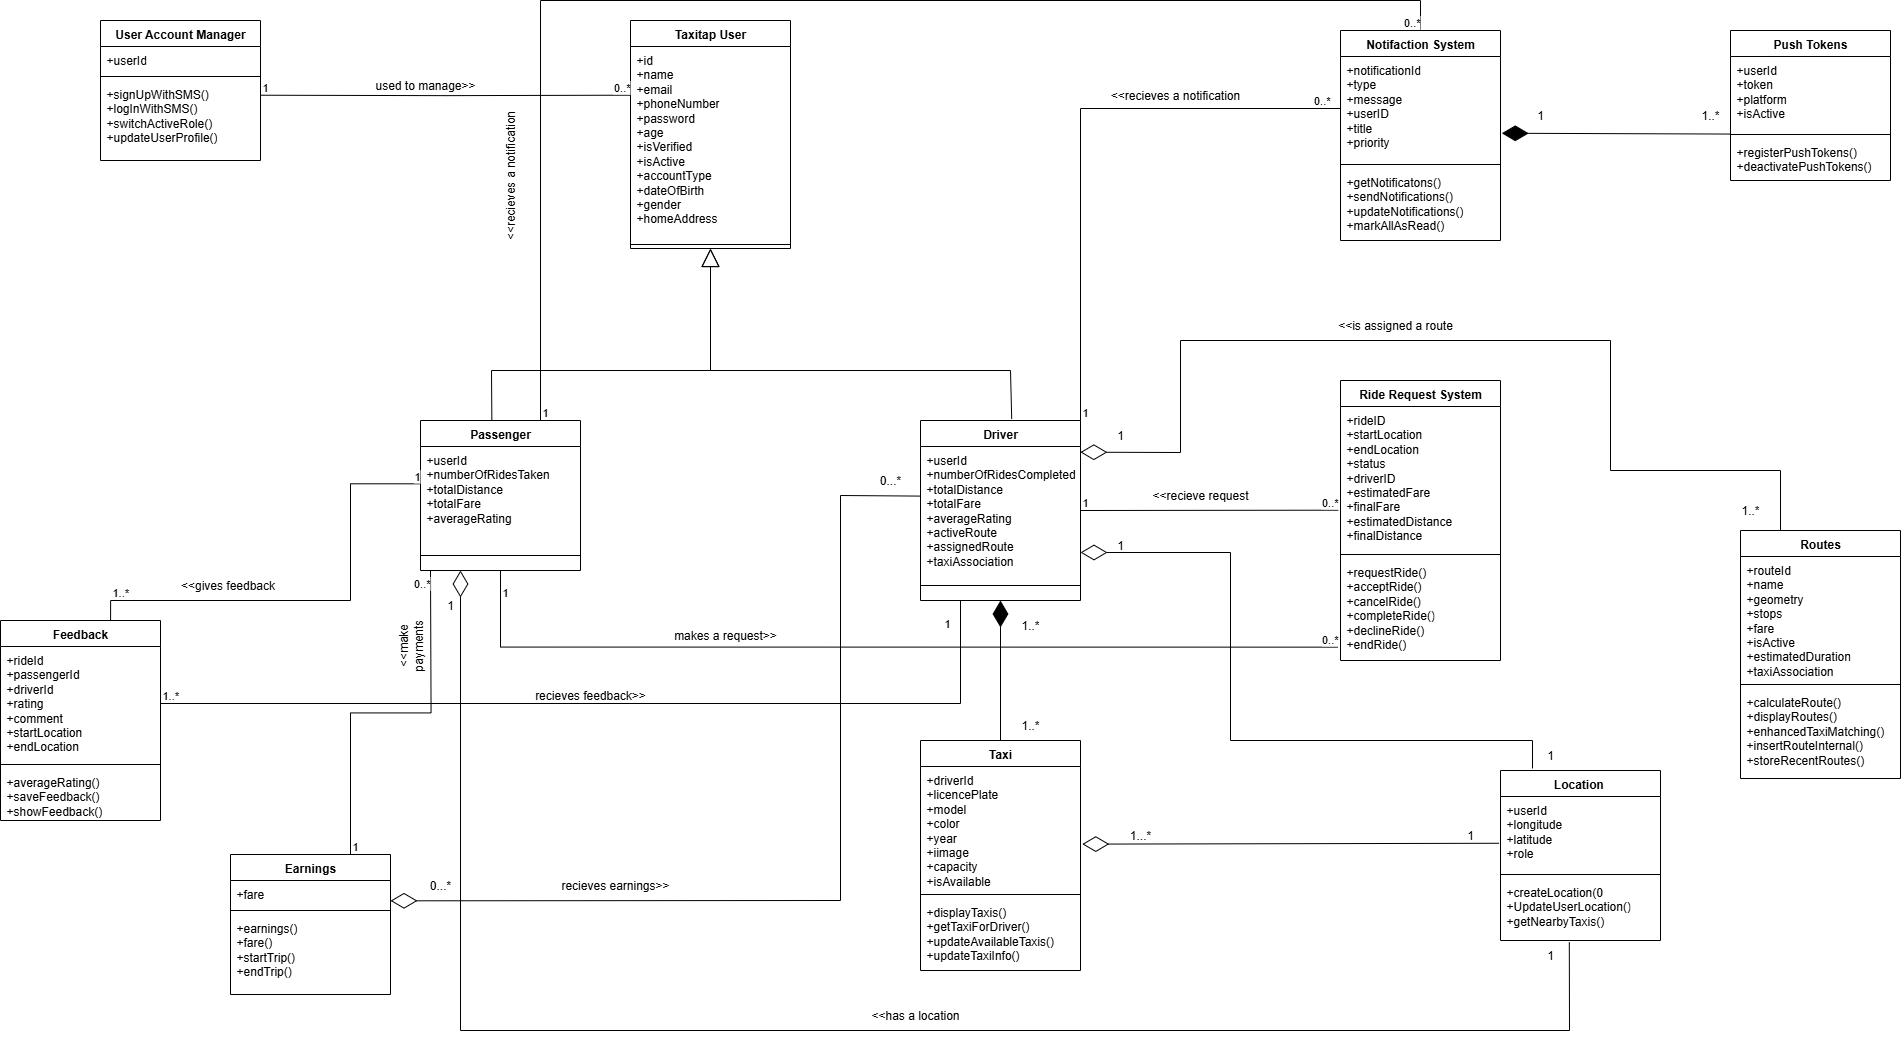
\includegraphics[width=1\textwidth]{Updated_Domain_Model.drawio.png} 
\end{figure}

\section{Functional Requirements}

\subsection*{R1: User Account Management}
\begin{itemize}
    \item R1.1: Users should be able to register as either a driver or a passenger.
    \item R1.2: Users should be able to update their Profile information.
    \item R1.3: The system should support role-based access control for passenger and driver interfaces.
    \item R1.4: Users should be able to reset or change their passwords.
    \item R1.5: Users should be able to switch between being a driver and a passenger.
\end{itemize}

\subsection*{R2: Location Services}
\begin{itemize}
    \item R2.1: The system should track driver locations in real-time using GPS.
    \item R2.2: The system should determine passenger locations for pickup requests.
    \item R2.3: The system should calculate proximity between taxis and passengers.
    \item R2.4: The system should send proximity alerts to notify passengers when their requested taxi is approaching.
    \item R2.5: The system should display estimated time of arrival for approaching taxis.
\end{itemize}

\subsection*{R3: Taxi Request System}
\begin{itemize}
    \item R3.1: Passengers should be able to request taxi pickups based on their location.
    \item R3.2: Passengers should be able to see nearby available taxis.
    \item R3.3: Drivers should be notified of nearby passenger pickup requests.
    \item R3.4: Drivers should be able to accept or decline pickup requests.
    \item R3.5: Passengers should be able to specify their destinations.
\end{itemize}

\subsection*{R4: Route Management}
\begin{itemize}
    \item R4.1: The system should allow drivers to announce their routes.
    \item R4.2: The system should display taxi routes to passengers.
    \item R4.3: The system should allow drivers to indicate their destinations.
    \item R4.4: The system should support flexible drop-off points along routes.
    \item R4.5: The system should display route information in a visual format suitable for quick comprehension.
\end{itemize}

\subsection*{R5: Taxi Status Information}
\begin{itemize}
    \item R5.1: The system should display real-time taxi tracking showing vehicle location.
    \item R5.2: The system should show available seats in approaching taxis.
    \item R5.3: The system should allow drivers to update their seat availability status.
    \item R5.4: The system should indicate taxi status (en route, picking up, full, etc.).
\end{itemize}

\subsection*{R6: Notifications}
\begin{itemize}
    \item R6.1: The system should send push notifications for taxi proximity alerts.
    \item R6.2: The system should notify passengers when their requested taxi accepts or declines the pickup.
    \item R6.3: The system should notify drivers of new nearby passenger requests.
    \item R6.4: The system should provide ETA updates to waiting passengers.
    \item R6.5: The system should send notifications even with limited connectivity.
\end{itemize}

\subsection*{R7: Passenger Destination Management}
\begin{itemize}
    \item R7.1: The system should allow passengers to specify their drop-off locations.
\end{itemize}

\subsection*{R8: User Interface}
\begin{itemize}
    \item R8.1: The system should provide separate interfaces for passengers and drivers.
    \item R8.2: The system should offer a clean, easy-to-use interface with visual elements.
    \item R8.3: The system should support multiple South African languages. 
\end{itemize}

\subsection*{R9: Rating and Feedback}
\begin{itemize}
    \item R9.1: Passengers should be able to rate drivers/taxis.
    \item R9.2: The system should collect feedback on routes and service.
\end{itemize}

\subsection*{R10: Fare Management}
\begin{itemize}
    \item R10.1: The system should calculate fare estimates based on route and distance.
    \item R10.2: The system should support cash payment options.
    \item R10.3: The system should track payment status for trips.
\end{itemize}

\subsection*{R11: Taxi Identification}
\begin{itemize}
    \item R11.1: The system should provide unique identifiers for each taxi.
    \item R11.2: The system should support  pin-based taxi identification and verification.
    \item R11.3: The system should display taxi information (registration, operator) to passengers.
\end{itemize}

\subsection*{R12: Safety Features}
\begin{itemize}
    \item R12.1: The system should include emergency contact features.
\end{itemize}

\section{Use Case Diagrams}
  \subsection*{Overall System}
    \begin{figure}[H]
      \centering
      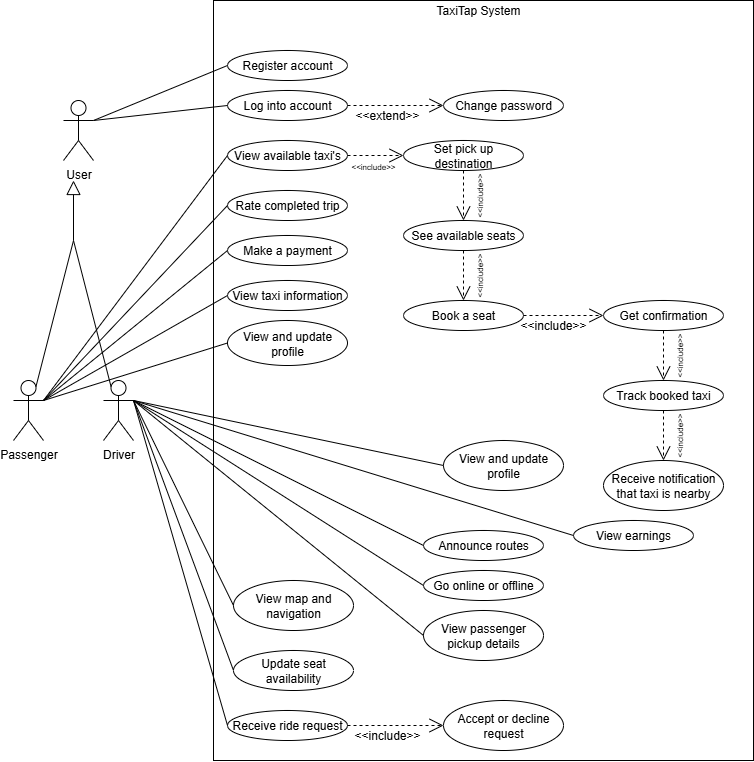
\includegraphics[width=1\textwidth]{Overall System.png} 
    \end{figure}
    \subsection*{Notification System}
    \begin{figure}[H]
      \centering
      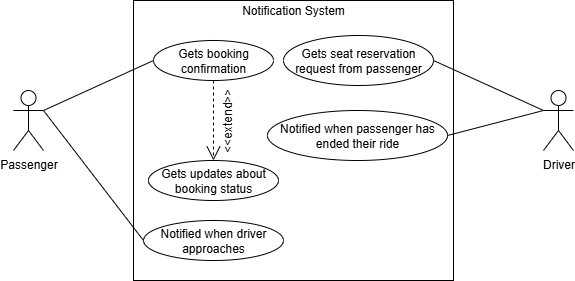
\includegraphics[width=1\textwidth]{Notification System.png} 
    \end{figure}
     \subsection*{Ride Request}
    \begin{figure}[H]
      \centering
      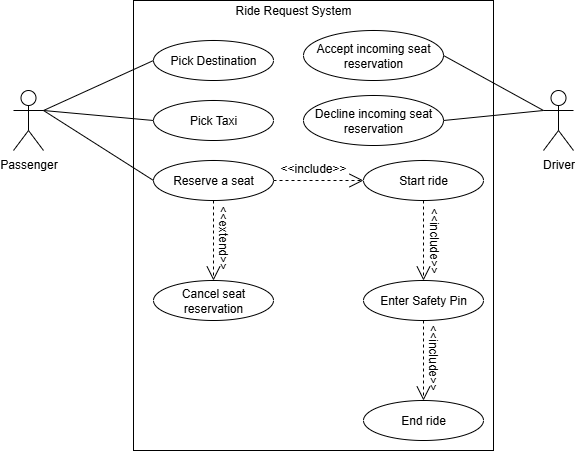
\includegraphics[width=1\textwidth]{Ride Request System.png} 
    \end{figure}
     \subsection*{Route Management System}
    \begin{figure}[H]
      \centering
      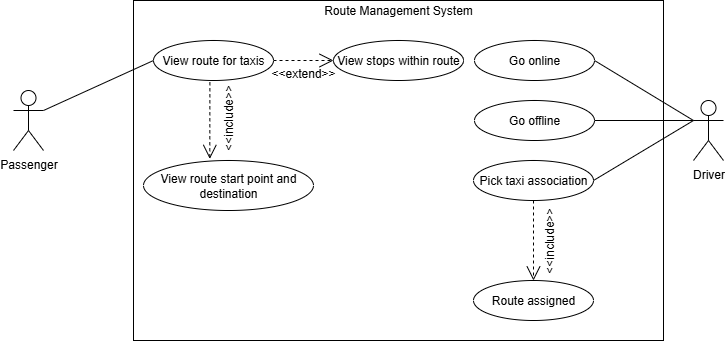
\includegraphics[width=1\textwidth]{Route Management System.png} 
    \end{figure}
    \subsection*{Location System}
    \begin{figure}[H]
      \centering
      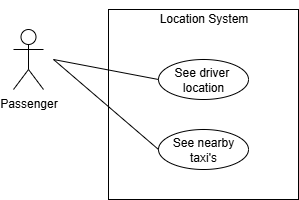
\includegraphics[width=0.7\textwidth]{Location System.png} 
    \end{figure}
   
  \subsection*{Feedback System}
    \begin{figure}[H]
      \centering
      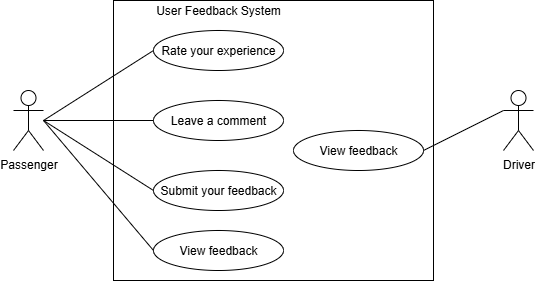
\includegraphics[width=1\textwidth]{Feedback.png} 
    \end{figure}
  \subsection*{Login System}
    \begin{figure}[H]
      \centering
      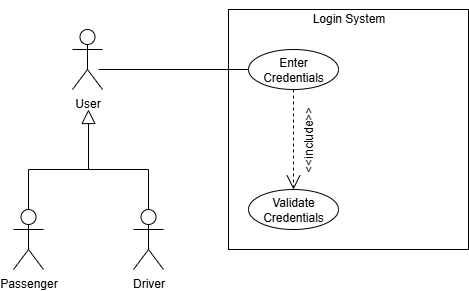
\includegraphics[width=1\textwidth]{Login System.png} 
    \end{figure}
  \subsection*{Signup System}
    \begin{figure}[H]
      \centering
      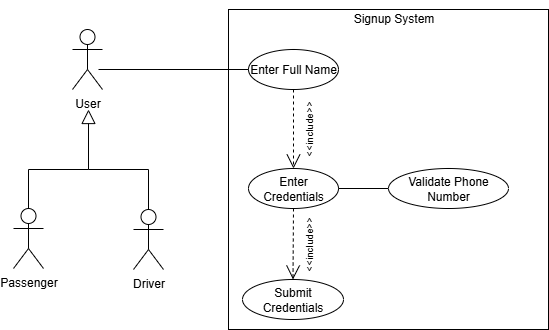
\includegraphics[width=1\textwidth]{Signup System.png} 
    \end{figure}
  \subsection*{Payment System}
    \begin{figure}[H]
      \centering
      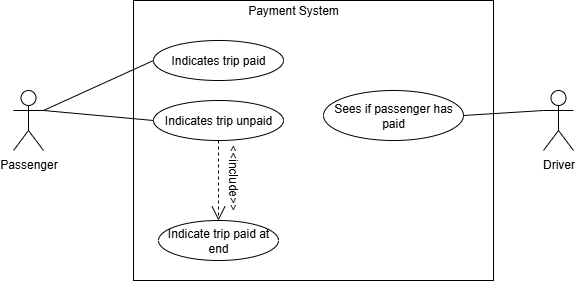
\includegraphics[width=1\textwidth]{Payment System.png} 
    \end{figure}

\section{Technology Requirements}

\subsection{Frontend}
\textbf{Expo (React Native with TypeScript)}\\
\textbf{Why we chose to use Expo?}
\begin{itemize}
    \item \textbf{Cross-platform Compatibility:} Code once, deploy to both Android and iOS.
    \item \textbf{Native Features:} Access to GPS, accelerometer, push notifications, offline storage, camera, QR scanning, etc.
    \item \textbf{Web Support:} Leverages Expo Web for rendering web-based dashboards and admin panels.
    \item \textbf{Live Reloading \& Fast Iteration:} Expo Go provides hot reloading and rapid prototyping with a unified development experience.
    \item \textbf{Battery \& Data Optimization:} React Native ecosystem provides fine-grained control over performance, reducing overhead.
\end{itemize}

\subsection{Backend}
\textbf{Convex (TypeScript)}\\
\textbf{Why we chose to use Convex?}
\begin{itemize}
    \item \textbf{Truly Serverless:} No provisioning, no scaling headaches. Functions, database, and auth all run in one integrated environment.
    \item \textbf{Built-in Database:} Convex provides a powerful document-oriented database that supports relations, IDs, indexes, and real-time reactivity.
    \item \textbf{Type Safety:} Schema definition is in TypeScript, ensuring end-to-end type safety from backend to frontend.
    \item \textbf{Zero DevOps:} No need to manage infrastructure or containers. Deploy directly from your project.
    \item \textbf{Realtime Sync:} Built-in support for reactive queries allows passengers to see live taxi updates, seat availability, and ETA.
\end{itemize}

\subsubsection*{Convex Database Architecture}
\begin{itemize}
    \item \textbf{Document Store:} Convex uses collections of JSON-like documents, like MongoDB, but with built-in schema validation.
    \item \textbf{Indexes:} Automatic indexing on IDs and custom indexing for optimized query performance.
    \item \textbf{Relationships:} You can use Convex \texttt{v.id()} to reference documents between tables, ensuring referential integrity.
    \item \textbf{Realtime Subscriptions:} Query results update automatically when the underlying data changes.
\end{itemize}

\subsubsection*{Convex Free Tier (as of 2025)}
\begin{itemize}
    \item Compute: Up to 1 million function calls/month.
    \item Storage: 1 GB document data storage.
    \item Bandwidth: 5 GB of egress.
    \item Authentication: Integrated with third-party auth providers (Firebase Auth, Clerk, etc.).
    \item Deployment: 1 Production Deployment and 1 Dev Deployment per project.
\end{itemize}

\noindent Perfect for COS 301: Within budget, no surprise bills, and production-grade scalability.

\subsection{Key Functional Modules \& Implementation Plan}

\subsubsection*{User Management Subsystem}
\begin{itemize}
    \item Authentication: Convex Auth with Clerk or Firebase integration.
    \item Registration/Login: Role-based registration (passenger or driver) with schema enforcement.
    \item Profile Updates: Mutation to update user document with profile fields.
    \item Security: JWT-based session validation, encryption at rest and in transit.
\end{itemize}

\subsubsection*{Location Services Subsystem}
\begin{itemize}
    \item Driver Location: Periodic GPS updates using Expo Location API.
    \item Passenger Location: One-time or continuous tracking during trip.
    \item Proximity Alerts: Triggered from Convex using background function.
    \item ETA Calculation: Naive approach using Haversine distance and average speed (no Google Maps API due to cost).
\end{itemize}

\subsubsection*{Taxi Request Subsystem}
\begin{itemize}
    \item Request Workflow:
    \begin{itemize}
        \item Passenger sends request with pickup and destination location.
        \item Nearby drivers notified (push notification via Expo).
        \item Driver accepts or rejects request.
        \item Status changes handled in real time.
    \end{itemize}
\end{itemize}

\subsubsection*{Route Management Subsystem}
\begin{itemize}
    \item Driver Route Declaration: Input form for common route and destination.
    \item Passenger View: Map view of taxis on route and destinations.
    \item Optimized Routing (Optional): Historical route optimization using stored patterns (stretch goal).
\end{itemize}

\subsubsection*{Notification System}
\begin{itemize}
    \item Technology: Expo Notifications API.
    \item Use Cases:
    \begin{itemize}
        \item Taxi is approaching.
        \item Ride accepted or declined.
        \item Route changes or delays.
    \end{itemize}
    \item Offline Support: Caching notifications locally using AsyncStorage.
\end{itemize}

\subsubsection*{Safety and Fare Management Subsystem}
\begin{itemize}
    \item Fare Estimate: Static fare matrix per route (e.g., km-based fare slabs).
\end{itemize}

\subsection{Testing Frameworks}
\begin{itemize}
    \item Backend: Jest (unit and integration tests for Convex functions).
    \item Frontend: React Native Testing Library.
    \item Manual Testing: Device tests using Expo Go and emulators.
\end{itemize}

\subsection{CI/CD}
\begin{itemize}
    \item Convex Deployment: Triggered via GitHub Action or manual \texttt{npx convex dev} / \texttt{convex deploy}.
    \item Expo Deployment: Use \texttt{eas build} and \texttt{eas submit} for App Store/Play Store releases (app store releases might note take place).
    \item Linting \& Tests: Pre-commit lint checks with ESLint and Jest unit tests.
\end{itemize}

\subsection{Version Control}
\begin{itemize}
    \item GitHub repo with main and dev branches.
    \item Feature branches for each core module.
\end{itemize}

\subsection{Quality Requirements}
Quality requirements determine the overall quality of Taxi Tap by specifying criteria that define how well the system performs and behaves.\newline

The quality requirements mentioned below are overall, but our top 5 is specified in the architectural requirements document.

\begin{enumerate}
    \item \textbf{Security}
    \begin{itemize}
        \item \textbf{Encryption:} All data must be encrypted in transit and at rest using the best security practices.
        \item \textbf{Compliance:}
        \begin{itemize}
            \item Data capturing and storing must adhere to the POPI act.
            \item Ensure data privacy and consent handling.
        \end{itemize}
        \item \textbf{Secure authentication:} Users must authenticate securely, and sessions must be protected.
    \end{itemize}

    \item \textbf{Usability}
    \begin{itemize}
        \item \textbf{Simplicity:} The interface should be easy to use for people with varying levels of tech literacy.
        \item \textbf{Accessibility:} The use of clear labels, large tap targets and minimal steps to complete key tasks.
        \item \textbf{Feedback and error handling:} Provide real-time feedback for user actions, loading states and clear error messages when issues occur.
    \end{itemize}

    \item \textbf{Scalability}
    \begin{itemize}
        \item The backend must scale to handle fluctuations in user or data load without performance degradation. This is automatically done by our chosen backend.
    \end{itemize}

    \item \textbf{Performance}
    \begin{itemize}
        \item \textbf{Low bandwidth optimization:} The system must perform reliably under low-bandwidth or intermittent connectivity.
        \item \textbf{Battery efficiency:} The app must minimize CPU, GPS and network usage to extend battery life.
    \end{itemize}

    \item \textbf{Reliability and Availability}
    \begin{itemize}
        \item \textbf{Offline Support:} The app must function even without a constant internet connection, using local caching or data queuing mechanisms.
        \item \textbf{High uptime:} The system should be available with minimal downtime to support driver operations throughout the day.
        \item \textbf{Data integrity:} Ensure that data is not lost or duplicated during sync offline and online states.
    \end{itemize}

    \item \textbf{Maintainability and Extensibility}
    \begin{itemize}
        \item \textbf{Clean architecture:} Backend and frontend systems should be modular and loosely coupled to allow easier updates, fixes, or feature additions in the future.
        \item \textbf{Logging and monitoring:} Implement centralized logging and monitoring to quickly identify and resolve issues.
        \item \textbf{Configurability:} Support code configurations without needing code changes.
    \end{itemize}

    \item \textbf{Affordability}
    \begin{itemize}
        \item \textbf{Low data consumption:} The app must use data sparingly to remain cost-effective for users in regions with expensive or limited mobile data.
        \item \textbf{Resource efficiency:} The system should minimize server and client-side consumption to reduce infrastructure and battery costs.
    \end{itemize}
\end{enumerate}

\subsection{Design Patterns}

\paragraph{Observer Pattern}
\begin{itemize}
    \item Pattern Type: Behavioural
    \item Participants:
    \begin{itemize}
        \item Subject: Notification System
        \item Observer: User
        \item Concrete Observer: Passenger, Driver 
    \end{itemize}
    \item Explanation: The Observer pattern allows an object (User) to be notified automatically of state changes in another object (Notification System). This is ideal for handling events like route updates or ride status.
    \item Example:
    \begin{itemize}
        \item User receives alerts from the Notification System.
        \item Notification System initiates a notification when a route is announced.
    \end{itemize}
\end{itemize}

\paragraph{Mediator Pattern}
\begin{itemize}
    \item Pattern Type: Behavioural
    \item Participants:
    \begin{itemize}
        \item Mediator: Taxi Request System
        \item Colleague: Passenger, Driver
    \end{itemize}
    \item Explanation: The Mediator pattern centralizes complex communication between objects. Instead of Passenger directly interacting with Driver, requests are handled through the Taxi Request System.
    \item Example:
    \begin{itemize}
        \item Taxi Request System acts as an intermediary between Passenger and Driver.
        \item Passenger makes a request for pickup to a driver, but the Taxi request system acts as the middleman for this request.
    \end{itemize}
\end{itemize}

\subsection{Constraints}
The client laid out the following constraints, by which Taxi Tap must abide, in their specification.

\begin{enumerate}
    \item \textbf{All data must be encrypted at transit and at rest}\\
    All data exchanged between the mobile application and backend services will be encrypted using HTTPS with TLS (Transport Layer Security). Role-based access policies and authentication mechanisms (e.g., JWTs) ensure only authorised users can access specific system resources.

    \item \textbf{POPI act}\\
    To ensure we abide by this, we will not collect any user data that is not necessary for the functionality of the app. With that, we will have permission set up to ensure that users are comfortable with collecting info, such as the user’s location. Furthermore, we will consider providing a Terms and Conditions for the app that lays out how user data will be used.

    \item \textbf{The app must function with low bandwidth, low data usage and be battery-efficient}\\
    We will accomplish this by having a UI that does not use too many resources and lightweight calls to the API.

    \item \textbf{Budget}\\
    We must use AWS Free Tier platforms or any platforms that are open source or within free tier allowance.
\end{enumerate}
\end{document}